\subsection{Wellen am Doppelspalt} \label{subsec:doppelspalt}

Wenn nun eine räumlich und zeitlich kohärente Wellen, das heißt Wellenfronten deren Wellen sowohl parallel als auch phasengleich (mit derselben Wellenlänge und Gangunterschied $\delta= k \cdot \lambda$) verlaufen, auf ein Hindernis mit 2 schmalen Spalten trifft, bildet sich folgendes Interferenzmuster:

%\begin{figure}[h!]
%	\center
%	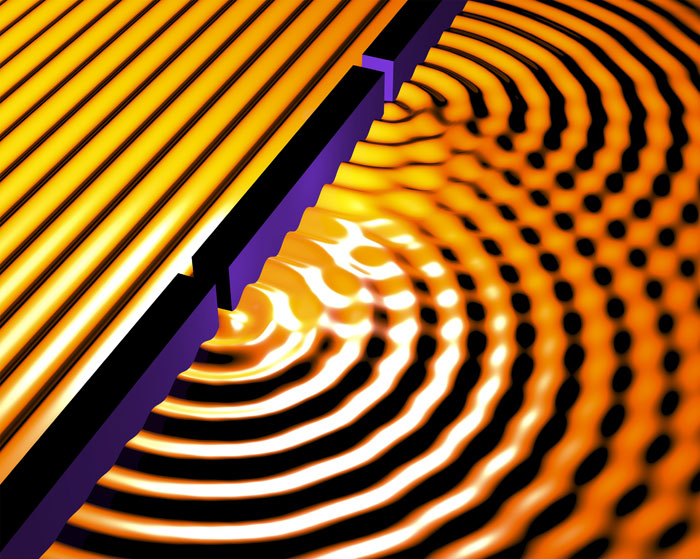
\includegraphics[width=0.4\textwidth]{doppelspalt_wasser}
%	\caption{Eine kohärente Welle am Doppelspalt}
%\end{figure}

Dies ist mit dem Huygens'schen Prinzip (\referenz{subsec:ausbreitung}) zu erklären: Angenommen, in jedem Spalt gäbe es nur ein schwingendes Teilchen. Dieses wird von der Wellenfront erfasst und ist selber Auslöser einer zirkularen Wellen. Da dieser Oszillator an dieser Stelle der einzige ist, gibt es keine gerade Wellenfront als Einhüllende, sondern einzig die Zirkularwelle des angeregten Oszillators.


\subsubsection{Mathematisierung}

	Der Versuch ist auch mit Laserlicht, also Monochromatisch (eine einzige Wellenlänge) und Kohärent, durchführbar. Das Licht wird durch einen schmalen Doppelspalt mit dem Spaltabstand $d \leq 2mm$ hinter dem sich im Abstand $a$ ein Schirm befindet. 
	
	Auf dem Schirm ist ein Interferenzmuster zu beobachten. In der Mitte ist ein heller Streifen, links und rechts davon, symmetrisch, sind weniger intensive Lichtpunkte. Diese Punkte werden Maxima genannt, da in diesen Punkten konstruktive Interferenz herrscht (\referenz{sec:interferenz}). An den Minimalstellen herrschen destruktive Interferenzen. Der Gangunterschied ergibt sich hier durch den Unterschiedlichen Abstand der Punkte auf dem Schirm zu dem beiden Schlitzen.
	
	Eine Zeichnung:
	
%	\begin{figure}[h!]
%		\center
%		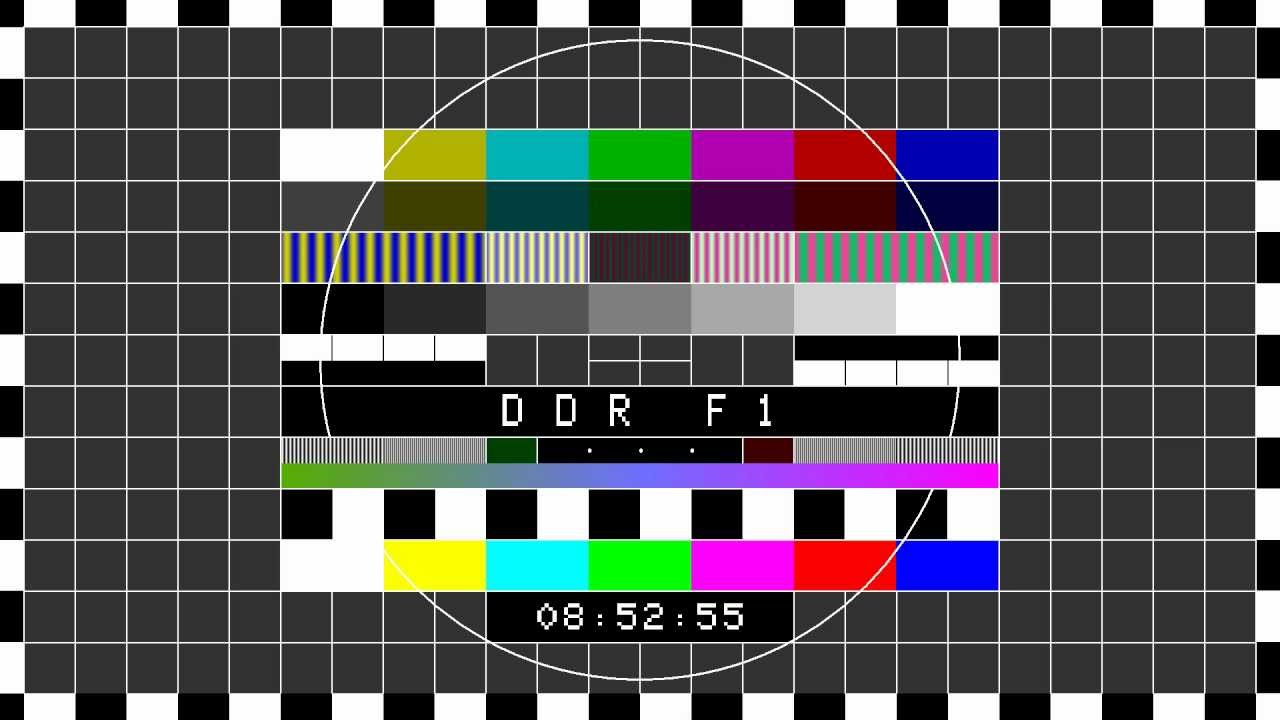
\includegraphics[width=0.8\textwidth]{default}
%		\caption{Das Maxima 1. Ordnung am Doppelspalt}
%	\end{figure}
	
	Die Winkel $\alpha_a$ und $\alpha_d$ sind gleich und werden im Folgen schlicht als $\alpha$ bezeichnet. Für $\alpha$ ergeben sich aus den trigonomischen Winkelfunktionen im rechtwinkligen Dreieck 2 Gleichungen: $sin{\alpha}=\frac{\delta}{d}$ und $tan{\alpha}=\frac{d_k}{a}$. Da $a>>d_k$ ist $\alpha<10 \degree$ und die Kleinwinkelnäherung $sin{\alpha} \approx \tan{alpha}$ kann verwendet werden. Der Gangunterschied $\delta$ muss der Bedingung für konstruktive Interferenz $\delta = k \cdot \lambda$ genügen (Siehe Gleichung \ref{eq:kon_interferenz} auf Seite \pageref{eq:kon_interferenz}). Daraus Ergibt sich:
	
	\begin{align}
		\sin{\alpha} &= \tan{\alpha} \\
		\frac{\delta}{d} &= \frac{d_k}{a} \\
		\frac{k \cdot \lambda}{d} &= \frac{d_k}{a}  \ \ \ wobei \ \ k \in 1,2,3... \\
		\lambda &= \frac{d_{k} \cdot d}{a \cdot k}  \ \ \ wobei \ \ k \in 1,2,3...
	\end{align}
	
	Für $k$ muss die Ordnung des betrachteten Maxima eingesetzt werden.
		

\subsubsection{Ohne Kleinwinkelnäherung}

	Um präziser ablesen zu können, kann ein Gitter statt einem Doppelspalt verwendet werden. Das Gitter weist einen wesentlich geringeren Abstand zwischen den Schlitzen auf (z.B. $\frac{1}{600}mm$), sodass die Interferenzmaxima deutlich weiter auseinander liegen. Der Fakt, dass der Lichtdurchsatz durch das Hinzufügen von mehr Schlitzen zu einem Gitter erhöht wurde, ändert nichts an den mathematischen Grundlagen des Versuchs.
	
	Allerdings geht mit dem größeren Abstand der Punkte auf dem Schirm die Gültigkeit der Kleinwinkelnäherung verloren. Allerdings kann die Größe des Winkels $\alpha_a$ über $\arctan{\frac{d_k}{a}}$ berechnet werden und in die Gleichung $\sin{\alpha} = \frac{\delta}{d}$ eingesetzt werden:
	
	\begin{align}
		\frac{\delta}{d} &= \sin{\alpha} \\
		 \delta &= \sin{(\arctan{\frac{d_k}{a}})} \cdot d \\
		\lambda \cdot k &= \sin{(\arctan{\frac{d_k}{a}})} \cdot d \ \ \ wobei \ \ k \in 1,2,3... \\
		\lambda &= \frac{\sin{(\arctan{\frac{d_k}{a}})} \cdot d}{k} \ \ \ wobei \ \ k \in 1,2,3...
	\end{align}


\subsection{Lichtspektrum am Doppelspalt}

Wenn ein Lichtspektrum (z.B. weißes Licht von einer Glühbirne) auf einen Doppelspalt oder ein Gitter trifft, dann tritt dasselbe Phänomen wie bei monochromatischem Licht, mit dem Unterschied, dass die unterschiedlichen Wellenlängen im Spektrum ihren eigenen, von der Wellenlänge abhängigen, Abstand $d_k$ haben. Dadurch wird das Lichtspektrum von violett bis rot aufgefächert (Dispersion).